\documentclass{standalone}
\usepackage{tikz}
\usetikzlibrary{patterns, positioning}
\usepackage[sfdefault]{ClearSans} %% option 'sfdefault' activates Clear Sans as the default text font
\usepackage[T1]{fontenc}

\begin{document}
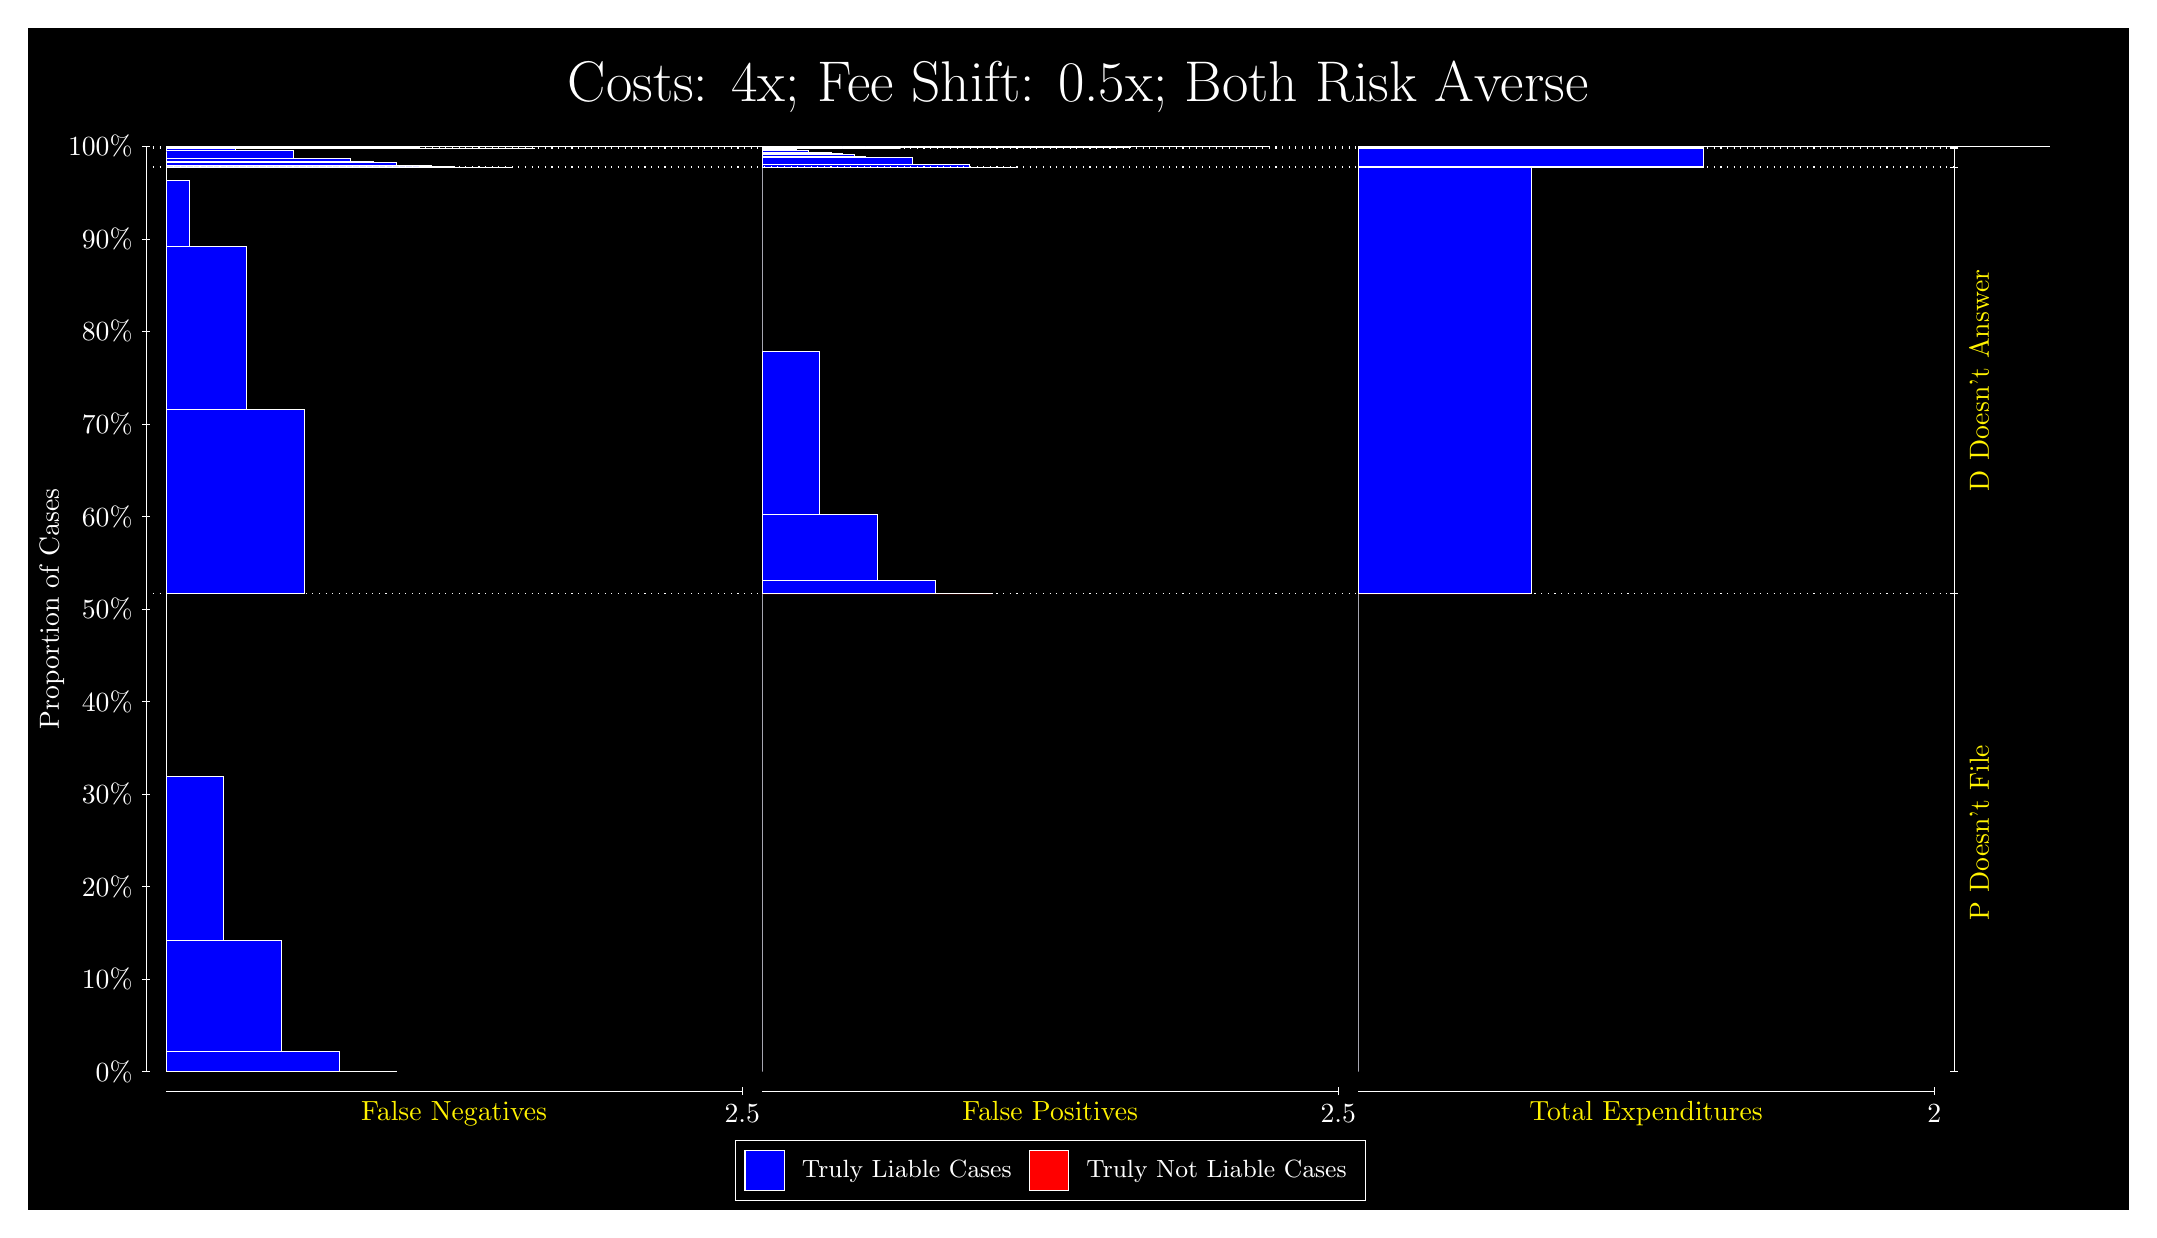
\begin{tikzpicture}
\draw[fill=black] (0,0) rectangle (26.667,15);
\draw[text=white] (0,13.5) rectangle (26.667,15) node[midway] {\huge Costs: 4x; Fee Shift: 0.5x; Both Risk Averse};
\draw[white, very thin] (1.5,1.75) -- (1.5,13.5);
\node[rotate=90, text=white, anchor=center] at (0.3, 7.625) {Proportion of Cases};
\draw[white, very thin] (1.45,1.75) -- (1.55,1.75);
\node[text=white, anchor=east] at (1.45, 1.75) {0\%};
\draw[white, very thin] (1.45,2.925) -- (1.55,2.925);
\node[text=white, anchor=east] at (1.45, 2.925) {10\%};
\draw[white, very thin] (1.45,4.1) -- (1.55,4.1);
\node[text=white, anchor=east] at (1.45, 4.1) {20\%};
\draw[white, very thin] (1.45,5.275) -- (1.55,5.275);
\node[text=white, anchor=east] at (1.45, 5.275) {30\%};
\draw[white, very thin] (1.45,6.45) -- (1.55,6.45);
\node[text=white, anchor=east] at (1.45, 6.45) {40\%};
\draw[white, very thin] (1.45,7.625) -- (1.55,7.625);
\node[text=white, anchor=east] at (1.45, 7.625) {50\%};
\draw[white, very thin] (1.45,8.8) -- (1.55,8.8);
\node[text=white, anchor=east] at (1.45, 8.8) {60\%};
\draw[white, very thin] (1.45,9.975) -- (1.55,9.975);
\node[text=white, anchor=east] at (1.45, 9.975) {70\%};
\draw[white, very thin] (1.45,11.15) -- (1.55,11.15);
\node[text=white, anchor=east] at (1.45, 11.15) {80\%};
\draw[white, very thin] (1.45,12.325) -- (1.55,12.325);
\node[text=white, anchor=east] at (1.45, 12.325) {90\%};
\draw[white, very thin] (1.45,13.5) -- (1.55,13.5);
\node[text=white, anchor=east] at (1.45, 13.5) {100\%};

\draw[white, very thin] (24.457,1.75) -- (24.457,13.5);
\draw[white, very thin] (24.407,1.75) -- (24.507,1.75);
\node[anchor=west] at (24.407, 1.75) {};
\draw[white, very thin] (24.407,7.8177) -- (24.507,7.8177);
\node[anchor=west] at (24.407, 7.8177) {};
\draw[white, very thin] (24.407,13.238) -- (24.507,13.238);
\node[anchor=west] at (24.407, 13.238) {};
\draw[white, very thin] (24.407,13.477) -- (24.507,13.477);
\node[anchor=west] at (24.407, 13.477) {};
\draw[white, very thin] (24.407,13.489) -- (24.507,13.489);
\node[anchor=west] at (24.407, 13.489) {};
\draw[white, very thin] (24.407,13.499) -- (24.507,13.499);
\node[anchor=west] at (24.407, 13.499) {};
\draw[white, very thin] (24.407,13.5) -- (24.507,13.5);
\node[anchor=west] at (24.407, 13.5) {};

\draw[white, very thin, fill=blue] (1.75,1.75) rectangle (4.6775,1.7525);
\draw[white, very thin, fill=blue] (1.75,1.7525) rectangle (3.9457,2.0022);
\draw[white, very thin, fill=blue] (1.75,2.0022) rectangle (3.2138,3.4142);
\draw[white, very thin, fill=blue] (1.75,3.4142) rectangle (2.4819,5.5052);
\draw[white, very thin, fill=red] (1.75,5.5052) rectangle (1.75,5.5052);
\draw[white, very thin, fill=blue] (1.75,5.5052) rectangle (1.75,7.8177);
\draw[white, very thin, fill=blue] (1.75,7.8177) rectangle (3.5065,10.165);
\draw[white, very thin, fill=blue] (1.75,10.165) rectangle (2.7746,12.229);
\draw[white, very thin, fill=blue] (1.75,12.229) rectangle (2.0428,13.067);
\draw[white, very thin, fill=red] (1.75,13.067) rectangle (1.75,13.067);
\draw[white, very thin, fill=blue] (1.75,13.067) rectangle (1.75,13.238);
\draw[white, very thin, fill=blue] (1.75,13.238) rectangle (6.1413,13.238);
\draw[white, very thin, fill=blue] (1.75,13.238) rectangle (5.8486,13.238);
\draw[white, very thin, fill=blue] (1.75,13.238) rectangle (5.5558,13.238);
\draw[white, very thin, fill=blue] (1.75,13.238) rectangle (5.4094,13.241);
\draw[white, very thin, fill=blue] (1.75,13.241) rectangle (5.1167,13.253);
\draw[white, very thin, fill=blue] (1.75,13.253) rectangle (4.9703,13.253);
\draw[white, very thin, fill=blue] (1.75,13.253) rectangle (4.8239,13.262);
\draw[white, very thin, fill=blue] (1.75,13.262) rectangle (4.6775,13.293);
\draw[white, very thin, fill=blue] (1.75,13.293) rectangle (4.3848,13.305);
\draw[white, very thin, fill=blue] (1.75,13.305) rectangle (4.2384,13.312);
\draw[white, very thin, fill=blue] (1.75,13.312) rectangle (4.092,13.347);
\draw[white, very thin, fill=blue] (1.75,13.347) rectangle (3.9457,13.349);
\draw[white, very thin, fill=blue] (1.75,13.349) rectangle (3.6529,13.349);
\draw[white, very thin, fill=blue] (1.75,13.349) rectangle (3.5065,13.353);
\draw[white, very thin, fill=blue] (1.75,13.353) rectangle (3.3602,13.445);
\draw[white, very thin, fill=blue] (1.75,13.445) rectangle (3.2138,13.445);
\draw[white, very thin, fill=blue] (1.75,13.445) rectangle (2.921,13.445);
\draw[white, very thin, fill=blue] (1.75,13.445) rectangle (2.7746,13.445);
\draw[white, very thin, fill=blue] (1.75,13.445) rectangle (2.6283,13.477);
\draw[white, very thin, fill=blue] (1.75,13.477) rectangle (2.0428,13.477);
\draw[white, very thin, fill=red] (1.75,13.477) rectangle (1.75,13.477);
\draw[white, very thin, fill=blue] (1.75,13.477) rectangle (6.4341,13.477);
\draw[white, very thin, fill=blue] (1.75,13.477) rectangle (5.7022,13.478);
\draw[white, very thin, fill=blue] (1.75,13.478) rectangle (4.9703,13.488);
\draw[white, very thin, fill=blue] (1.75,13.488) rectangle (4.2384,13.489);
\draw[white, very thin, fill=blue] (1.75,13.489) rectangle (3.5065,13.489);
\draw[white, very thin, fill=red] (1.75,13.489) rectangle (1.75,13.489);
\draw[white, very thin, fill=blue] (1.75,13.489) rectangle (3.5065,13.489);
\draw[white, very thin, fill=blue] (1.75,13.489) rectangle (2.7746,13.493);
\draw[white, very thin, fill=blue] (1.75,13.493) rectangle (2.0428,13.498);
\draw[white, very thin, fill=red] (1.75,13.498) rectangle (1.75,13.498);
\draw[white, very thin, fill=blue] (1.75,13.498) rectangle (1.75,13.499);
\draw[white, very thin, fill=blue] (1.75,13.499) rectangle (9.9471,13.499);
\draw[white, very thin, fill=blue] (1.75,13.499) rectangle (9.2152,13.499);
\draw[white, very thin, fill=blue] (1.75,13.499) rectangle (8.4834,13.499);
\draw[white, very thin, fill=blue] (1.75,13.499) rectangle (7.7515,13.499);
\draw[white, very thin, fill=blue] (1.75,13.499) rectangle (7.4587,13.499);
\draw[white, very thin, fill=blue] (1.75,13.499) rectangle (7.0196,13.499);
\draw[white, very thin, fill=blue] (1.75,13.499) rectangle (6.7268,13.499);
\draw[white, very thin, fill=blue] (1.75,13.499) rectangle (6.2877,13.499);
\draw[white, very thin, fill=blue] (1.75,13.499) rectangle (5.9949,13.499);
\draw[white, very thin, fill=blue] (1.75,13.499) rectangle (5.2631,13.5);
\draw[white, very thin, fill=blue] (1.75,13.5) rectangle (4.5312,13.5);
\draw[white, very thin, fill=blue] (1.75,13.5) rectangle (3.7993,13.5);
\draw[white, very thin, fill=blue] (1.75,13.5) rectangle (3.0674,13.5);
\draw[white, very thin, fill=blue] (1.75,13.5) rectangle (2.3355,13.5);
\draw[white, very thin, fill=red] (1.75,13.5) rectangle (1.75,13.5);
\draw[white, very thin, fill=red] (9.3189,1.75) rectangle (9.3189,1.75);
\draw[white, very thin, fill=blue] (9.3189,1.75) rectangle (9.3189,7.8177);
\draw[white, very thin, fill=red] (9.3189,7.8177) rectangle (12.246,7.8177);
\draw[white, very thin, fill=blue] (9.3189,7.8177) rectangle (12.246,7.8227);
\draw[white, very thin, fill=blue] (9.3189,7.8227) rectangle (11.515,7.9884);
\draw[white, very thin, fill=blue] (9.3189,7.9884) rectangle (10.783,8.8267);
\draw[white, very thin, fill=blue] (9.3189,8.8267) rectangle (10.051,10.891);
\draw[white, very thin, fill=blue] (9.3189,10.891) rectangle (9.3189,13.238);
\draw[white, very thin, fill=red] (9.3189,13.238) rectangle (12.539,13.238);
\draw[white, very thin, fill=blue] (9.3189,13.238) rectangle (12.539,13.238);
\draw[white, very thin, fill=red] (9.3189,13.238) rectangle (11.954,13.238);
\draw[white, very thin, fill=blue] (9.3189,13.238) rectangle (11.954,13.27);
\draw[white, very thin, fill=blue] (9.3189,13.27) rectangle (11.807,13.27);
\draw[white, very thin, fill=red] (9.3189,13.27) rectangle (11.661,13.27);
\draw[white, very thin, fill=blue] (9.3189,13.27) rectangle (11.661,13.27);
\draw[white, very thin, fill=red] (9.3189,13.27) rectangle (11.368,13.27);
\draw[white, very thin, fill=blue] (9.3189,13.27) rectangle (11.368,13.27);
\draw[white, very thin, fill=blue] (9.3189,13.27) rectangle (11.222,13.362);
\draw[white, very thin, fill=blue] (9.3189,13.362) rectangle (11.075,13.366);
\draw[white, very thin, fill=blue] (9.3189,13.366) rectangle (10.929,13.366);
\draw[white, very thin, fill=blue] (9.3189,13.366) rectangle (10.636,13.368);
\draw[white, very thin, fill=blue] (9.3189,13.368) rectangle (10.49,13.403);
\draw[white, very thin, fill=blue] (9.3189,13.403) rectangle (10.344,13.41);
\draw[white, very thin, fill=blue] (9.3189,13.41) rectangle (10.197,13.422);
\draw[white, very thin, fill=blue] (9.3189,13.422) rectangle (9.9044,13.453);
\draw[white, very thin, fill=blue] (9.3189,13.453) rectangle (9.758,13.462);
\draw[white, very thin, fill=blue] (9.3189,13.462) rectangle (9.6116,13.462);
\draw[white, very thin, fill=blue] (9.3189,13.462) rectangle (9.4652,13.474);
\draw[white, very thin, fill=blue] (9.3189,13.474) rectangle (9.3189,13.477);
\draw[white, very thin, fill=red] (9.3189,13.477) rectangle (11.075,13.477);
\draw[white, very thin, fill=blue] (9.3189,13.477) rectangle (11.075,13.477);
\draw[white, very thin, fill=blue] (9.3189,13.477) rectangle (10.344,13.477);
\draw[white, very thin, fill=blue] (9.3189,13.477) rectangle (9.6116,13.487);
\draw[white, very thin, fill=blue] (9.3189,13.487) rectangle (9.3189,13.489);
\draw[white, very thin, fill=red] (9.3189,13.489) rectangle (14.003,13.489);
\draw[white, very thin, fill=blue] (9.3189,13.489) rectangle (14.003,13.489);
\draw[white, very thin, fill=blue] (9.3189,13.489) rectangle (13.271,13.489);
\draw[white, very thin, fill=blue] (9.3189,13.489) rectangle (12.539,13.495);
\draw[white, very thin, fill=blue] (9.3189,13.495) rectangle (11.807,13.499);
\draw[white, very thin, fill=blue] (9.3189,13.499) rectangle (11.075,13.499);
\draw[white, very thin, fill=red] (9.3189,13.499) rectangle (15.759,13.499);
\draw[white, very thin, fill=blue] (9.3189,13.499) rectangle (15.759,13.499);
\draw[white, very thin, fill=blue] (9.3189,13.499) rectangle (15.028,13.499);
\draw[white, very thin, fill=red] (9.3189,13.499) rectangle (15.028,13.499);
\draw[white, very thin, fill=blue] (9.3189,13.499) rectangle (15.028,13.499);
\draw[white, very thin, fill=blue] (9.3189,13.499) rectangle (14.296,13.499);
\draw[white, very thin, fill=red] (9.3189,13.499) rectangle (14.296,13.499);
\draw[white, very thin, fill=blue] (9.3189,13.499) rectangle (14.296,13.499);
\draw[white, very thin, fill=blue] (9.3189,13.499) rectangle (13.564,13.499);
\draw[white, very thin, fill=red] (9.3189,13.499) rectangle (13.564,13.499);
\draw[white, very thin, fill=blue] (9.3189,13.499) rectangle (13.564,13.499);
\draw[white, very thin, fill=blue] (9.3189,13.499) rectangle (12.832,13.499);
\draw[white, very thin, fill=blue] (9.3189,13.499) rectangle (12.832,13.5);
\draw[white, very thin, fill=blue] (9.3189,13.5) rectangle (12.1,13.5);
\draw[white, very thin, fill=red] (9.3189,13.5) rectangle (11.807,13.5);
\draw[white, very thin, fill=blue] (9.3189,13.5) rectangle (11.807,13.5);
\draw[white, very thin, fill=blue] (9.3189,13.5) rectangle (11.368,13.5);
\draw[white, very thin, fill=red] (9.3189,13.5) rectangle (11.075,13.5);
\draw[white, very thin, fill=blue] (9.3189,13.5) rectangle (11.075,13.5);
\draw[white, very thin, fill=blue] (9.3189,13.5) rectangle (10.636,13.5);
\draw[white, very thin, fill=blue] (9.3189,13.5) rectangle (10.344,13.5);
\draw[white, very thin, fill=blue] (9.3189,13.5) rectangle (9.6116,13.5);
\draw[white, very thin, fill=blue] (9.3189,13.5) rectangle (9.3189,13.5);
\draw[white, very thin, fill=red] (16.888,1.75) rectangle (16.888,1.75);
\draw[white, very thin, fill=blue] (16.888,1.75) rectangle (16.888,7.8177);
\draw[white, very thin, fill=red] (16.888,7.8177) rectangle (19.083,7.8177);
\draw[white, very thin, fill=blue] (16.888,7.8177) rectangle (19.083,13.238);
\draw[white, very thin, fill=red] (16.888,13.238) rectangle (21.279,13.238);
\draw[white, very thin, fill=blue] (16.888,13.238) rectangle (21.279,13.25);
\draw[white, very thin, fill=red] (16.888,13.25) rectangle (21.279,13.25);
\draw[white, very thin, fill=blue] (16.888,13.25) rectangle (21.279,13.477);
\draw[white, very thin, fill=red] (16.888,13.477) rectangle (21.279,13.477);
\draw[white, very thin, fill=blue] (16.888,13.477) rectangle (21.279,13.489);
\draw[white, very thin, fill=red] (16.888,13.489) rectangle (21.279,13.489);
\draw[white, very thin, fill=blue] (16.888,13.489) rectangle (21.279,13.499);
\draw[white, very thin, fill=red] (16.888,13.499) rectangle (25.67,13.499);
\draw[white, very thin, fill=blue] (16.888,13.499) rectangle (25.67,13.499);
\draw[white, very thin, fill=red] (16.888,13.499) rectangle (25.67,13.499);
\draw[white, very thin, fill=blue] (16.888,13.499) rectangle (25.67,13.5);
\draw[white, dotted] (1.5,7.8177) -- (24.457,7.8177);
\draw[white, dotted] (1.5,13.238) -- (24.457,13.238);
\draw[white, dotted] (1.5,13.477) -- (24.457,13.477);
\draw[white, dotted] (1.5,13.489) -- (24.457,13.489);
\draw[white, dotted] (1.5,13.499) -- (24.457,13.499);
\draw[white, very thin] (1.75,1.5) -- (9.0689,1.5);
\node[text=yellow, anchor=north] at (5.4094, 1.5) {False Negatives};
\draw[white, very thin] (9.0689,1.45) -- (9.0689,1.55);
\node[text=white, anchor=north] at (9.0689, 1.45) {2.5};

\draw[white, very thin] (9.3189,1.5) -- (16.638,1.5);
\node[text=yellow, anchor=north] at (12.978, 1.5) {False Positives};
\draw[white, very thin] (16.638,1.45) -- (16.638,1.55);
\node[text=white, anchor=north] at (16.638, 1.45) {2.5};

\draw[white, very thin] (16.888,1.5) -- (24.207,1.5);
\node[text=yellow, anchor=north] at (20.547, 1.5) {Total Expenditures};
\draw[white, very thin] (24.207,1.45) -- (24.207,1.55);
\node[text=white, anchor=north] at (24.207, 1.45) {2};

\node[text=yellow, centered, rotate=90] at (24.777, 4.7838) {P Doesn't File};
\node[text=yellow, centered, rotate=90] at (24.777, 10.528) {D Doesn't Answer};





\draw (12.978300999999998,1.5) node[draw=none] (baseCoordinate) {};
\begin{scope}[align=center]
        \matrix[scale=0.5, draw=white, below=0.5cm of baseCoordinate, nodes={draw}, column sep=0.1cm]{
            \node[rectangle, draw, minimum width=0.5cm, minimum height=0.5cm, fill=blue] {}; &
            \node[draw=none, font=\small, text=white] (B) {Truly Liable Cases}; &
            \node[rectangle, draw, minimum width=0.5cm, minimum height=0.5cm, fill=red] {}; &
            \node[draw=none, font=\small, text=white] (B) {Truly Not Liable Cases}; \\
            };
\end{scope}

\end{tikzpicture}
\end{document}